% ============================================================
%  深圳大学实验报告模板（SZU Experiment Report Template）
% This template can be modified according to the specific requirements of your experiment or project.
% Produced by: Chao Fan and Kewei Ou, AI School of SZU
% ============================================================

\documentclass[a4paper,12pt]{article}

% ----------------------------
% 中文与字体支持
% ----------------------------
\usepackage{fontspec}    % 字体支持
\usepackage{xeCJK}       % 中文字体支持
\IfFontExistsTF{Noto Serif CJK SC}
  {\setCJKmainfont{Noto Serif CJK SC}} % Overleaf
  {\setCJKmainfont{SimSun}}            % 本机回退字体

% ----------------------------
% 页面设置与常用宏包
% ----------------------------
\usepackage{geometry}    % 页面边距控制
\geometry{left=1in, right=1in, top=1in, bottom=1in}

\usepackage{longtable}   % 支持长表格
\usepackage{graphicx}    % 插入图片
\usepackage{fancyhdr}    % 页眉页脚控制
\usepackage{tikz}        % 绘制框线等图形
\usetikzlibrary{calc}    % 坐标计算
\usepackage{verbatim}    % 显示代码块
\usepackage{float}       % 控制图片浮动位置（[H]参数）
\usepackage{amsmath}     % 数学公式
\usepackage{booktabs}    % 三线表
\usepackage{array}       % 表格列格式
\usepackage{caption}     % 图表标题
\usepackage{setspace}    % 正文行距
\renewcommand{\figurename}{图}
\renewcommand{\tablename}{表}

% ----------------------------
% 页眉页脚设置
% ----------------------------
% \pagestyle{fancy}
\fancyhf{} % 清空默认页眉页脚
% \fancyhead[L]{深圳大学实验报告} % 左侧页眉文字
\fancyhead[C]{} % 中间空
\fancyhead[R]{} % 右侧空

% ============================================================
%                      文档开始
% ============================================================

\begin{document}

% ============================================================
% 封面页
% ============================================================
\begin{titlepage}
  \centering
  \vspace*{2cm}
  \Huge{\textbf{深 \ 圳 \ 大 \ 学 \ 实 \ 验  \ 报 \ 告}}\\[1.5cm]

  {\Large\textbf{课程名称}\quad\underline{\makebox[8cm][c]{Python程序设计}}}\\[0.5cm]
  {\Large
  \noindent\makebox[3.2cm][l]{\textbf{项目名称}}
  \underline{\makebox[8cm][c]{NumPy实现ViT图像编码器}}}\\[0.5cm]
  {\Large
  \noindent\makebox[3.2cm][l]{\textbf{学 \qquad 院}}
  \underline{\makebox[8cm][c]{人工智能学院}}}\\[0.5cm]
  {\Large
  \noindent\makebox[3.2cm][l]{\textbf{专 \qquad 业}}
  \underline{\makebox[8cm][c]{人工智能专业}}}\\[0.5cm]
  {\Large
  \noindent\makebox[3.2cm][l]{\textbf{指导教师}}
  \underline{\makebox[8cm][c]{樊超}}}\\[0.5cm]
  {\Large
  \noindent\makebox[3.2cm][l]{\textbf{\ 报 \ 告 \ 人}}
  \underline{\makebox[3cm][c]{余家铭}}
  \hspace{0.5cm}
  \textbf{学号}
  \underline{\makebox[3cm][c]{2025681055}}}\\[0.5cm]
  {\Large
  \noindent\makebox[3.2cm][l]{\textbf{实验时间}}
  \underline{\makebox[8cm][c]{2026年11月10日 周二}}}\\[0.5cm]
  {\Large
  \noindent\makebox[3.2cm][l]{\textbf{提交时间}}
  \underline{\makebox[8cm][c]{2026年11月11日 周三}}}\\[1.5cm]

  \vfill
  \Large{\textbf{教务处制}}
\end{titlepage}

\newpage
\setstretch{1.15}

% ============================================================
% 正文部分
% ============================================================
% Experiment Objectives


\section{实验目的}

本项目的目标是使用 NumPy 完成 OpenCLIP ViT-B/32 图像编码器的前向计算。
模型参数、图像预处理程序和参考结果由项目提供，不涉及模型训练。
编码器接收形状为 $[B,3,224,224]$ 的图像数组，
经过图像块划分、token 嵌入、12 层 Transformer 和输出投影，得到每张图像对应的 $512$ 维单位向量。

实验重点掌握 \texttt{reshape}、\texttt{transpose}、矩阵乘法和广播等 NumPy 操作；
理解多头注意力、残差连接及 MLP 的前向过程。调试完成后，利用提供的独立 FP32 参考数组验证各阶段计算结果。


% Experiment Process
\section{总体流程}
程序的整体数据流如图~\ref{fig:vit-arch} 所示，主要步骤如下：
\begin{enumerate}
  \item 将预处理后的图像按 $32\times32$ 划分为 $7\times7=49$ 个图像块，并将每个 RGB 图像块展平为 $3072$ 维向量；
  \item 将图像块投影到 $768$ 维，添加 CLS token 和位置嵌入，形成 $[B,50,768]$ 的 token 序列；
  \item 依次通过 12 个 Transformer 块，从最终序列中取出 CLS token，经后置归一化、$768\to512$ 投影和单位长度归一化得到输出。
\end{enumerate}

% Figure
\begin{figure}[t]
  \centering
  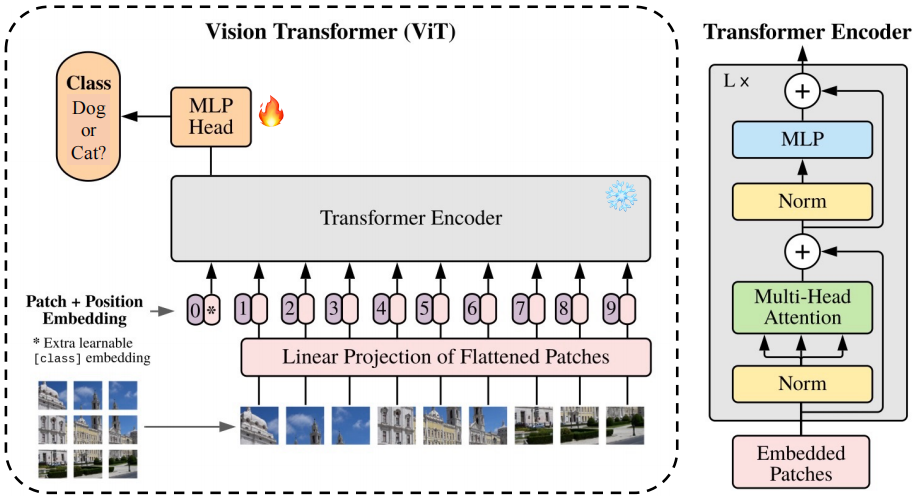
\includegraphics[width=0.92\linewidth]{figs/vit_overview.png}
  \caption{ViT 图像编码器的总体前向流程}
  \label{fig:vit-arch}
\end{figure}

% Implementation Details
\section{实验过程}
\subsection*{图像块划分与多头组织}

实验先从图像块划分开始。我先根据输入形状确定每张图像应分成 $7\times7$ 个 $32\times32$ 图像块，再将 $[B,3,224,224]$ 重排为 $[B,3,7,32,7,32]$。为了让同一位置的 RGB 数据保留在同一个图像块中，需要按以下顺序转置各轴：
\begin{center}
  \texttt{x = x.transpose(0,2,4,1,3,5)}
\end{center}
这样两个图像块网格轴位于通道轴之前，最后展平为 $[B,49,3072]$。
在调试时，我曾把通道轴合并到图像块数量中，结果却变成 147 个单通道小块。
随后搞清楚模型要求，我将排列修正为 $[B,7,7,3,32,32]$，才得到正确的 49 个 RGB 图像块。

多头部分采用同样的思路处理。
我们将 token 的 $768$ 维特征拆成 12 个注意力头，每个头包含 $64$ 维特征。
数组先由 $[B,N,D]$ 变成 $[B,N,H,D/H]$，再交换 token 轴与 head 轴，得到 $[B,H,N,D/H]$。

\begin{figure}[H]
  \centering
  \begin{minipage}[t]{0.49\linewidth}
    \centering
    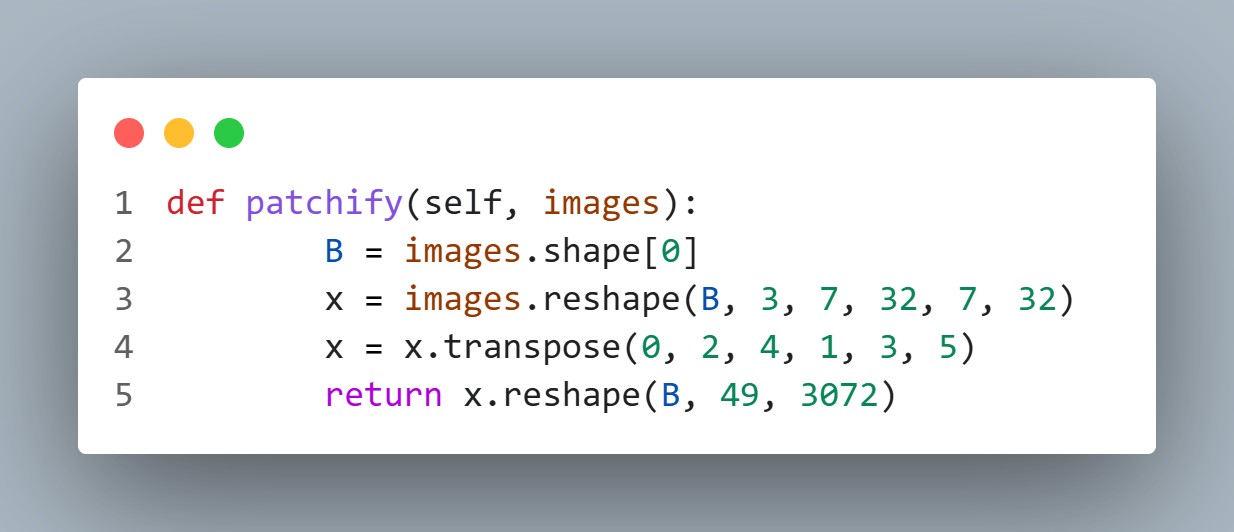
\includegraphics[width=\linewidth]{../image/todo1.png}
    \caption*{(a) TODO-01：图像块划分}
  \end{minipage}\hfill
  \begin{minipage}[t]{0.49\linewidth}
    \centering
    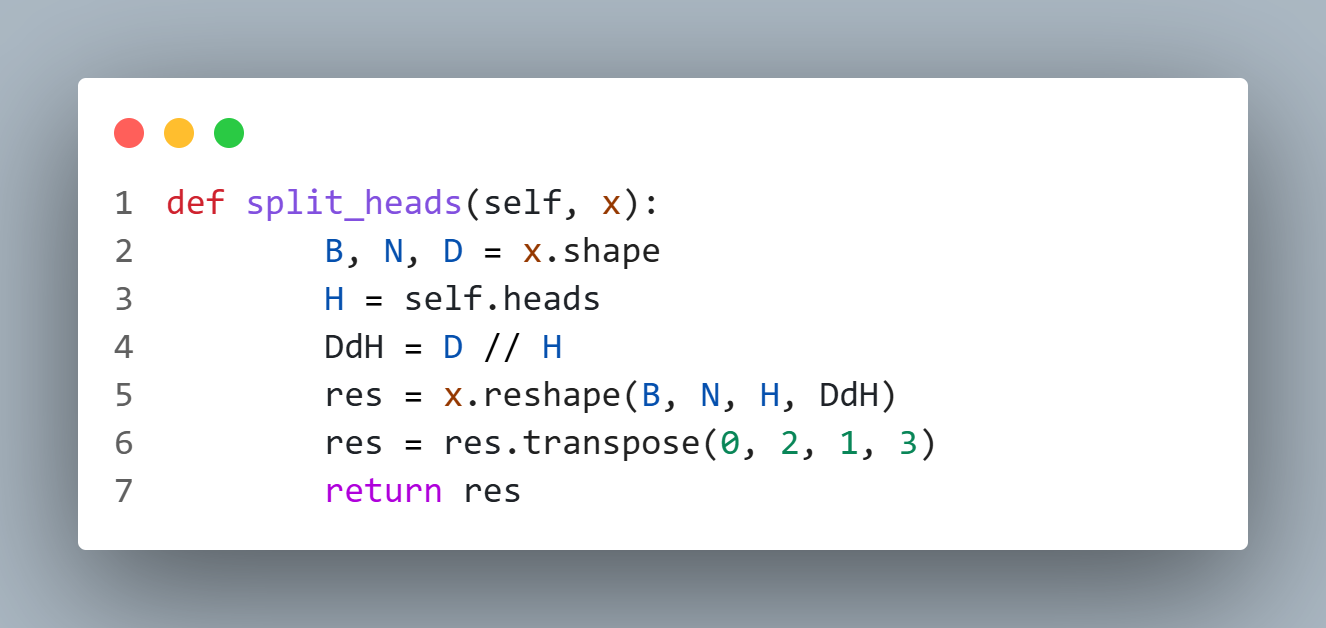
\includegraphics[width=\linewidth]{../image/todo2.png}
    \caption*{(b) TODO-02：拆分多头}
  \end{minipage}
  \caption{图像块划分与多头形状变换的实现}
  \label{fig:todo12}
\end{figure}

\subsection*{注意力与 Transformer 块}

完成拆头后，用点积缩放 $\dfrac{QK^{\mathsf T}}{\sqrt{d}}$ 计算形状为 $[B,H,N,N]$ 的注意力分数。
实际的 $K$ 是四维数组，因此我们只交换最后两个轴，保留 batch 和 head 的分组。
分数经过提供的 \texttt{attention\_weights} 转换为权重，再与 $V$ 相乘得到各头的上下文。
交换 head 与 token 轴，最后将 12 个头重新合并为 $[B,N,768]$ 并完成输出投影。

Transformer 块中保留了两条残差路径。第一次将注意力更新量加回原输入；
第二次对该结果进行 LayerNorm，再通过 $768\to3072\to768$ 的 MLP 和 GELU，最后将 MLP 更新量加回。

\begin{figure}[H]
  \centering
  \begin{minipage}[t]{0.49\linewidth}
    \centering
    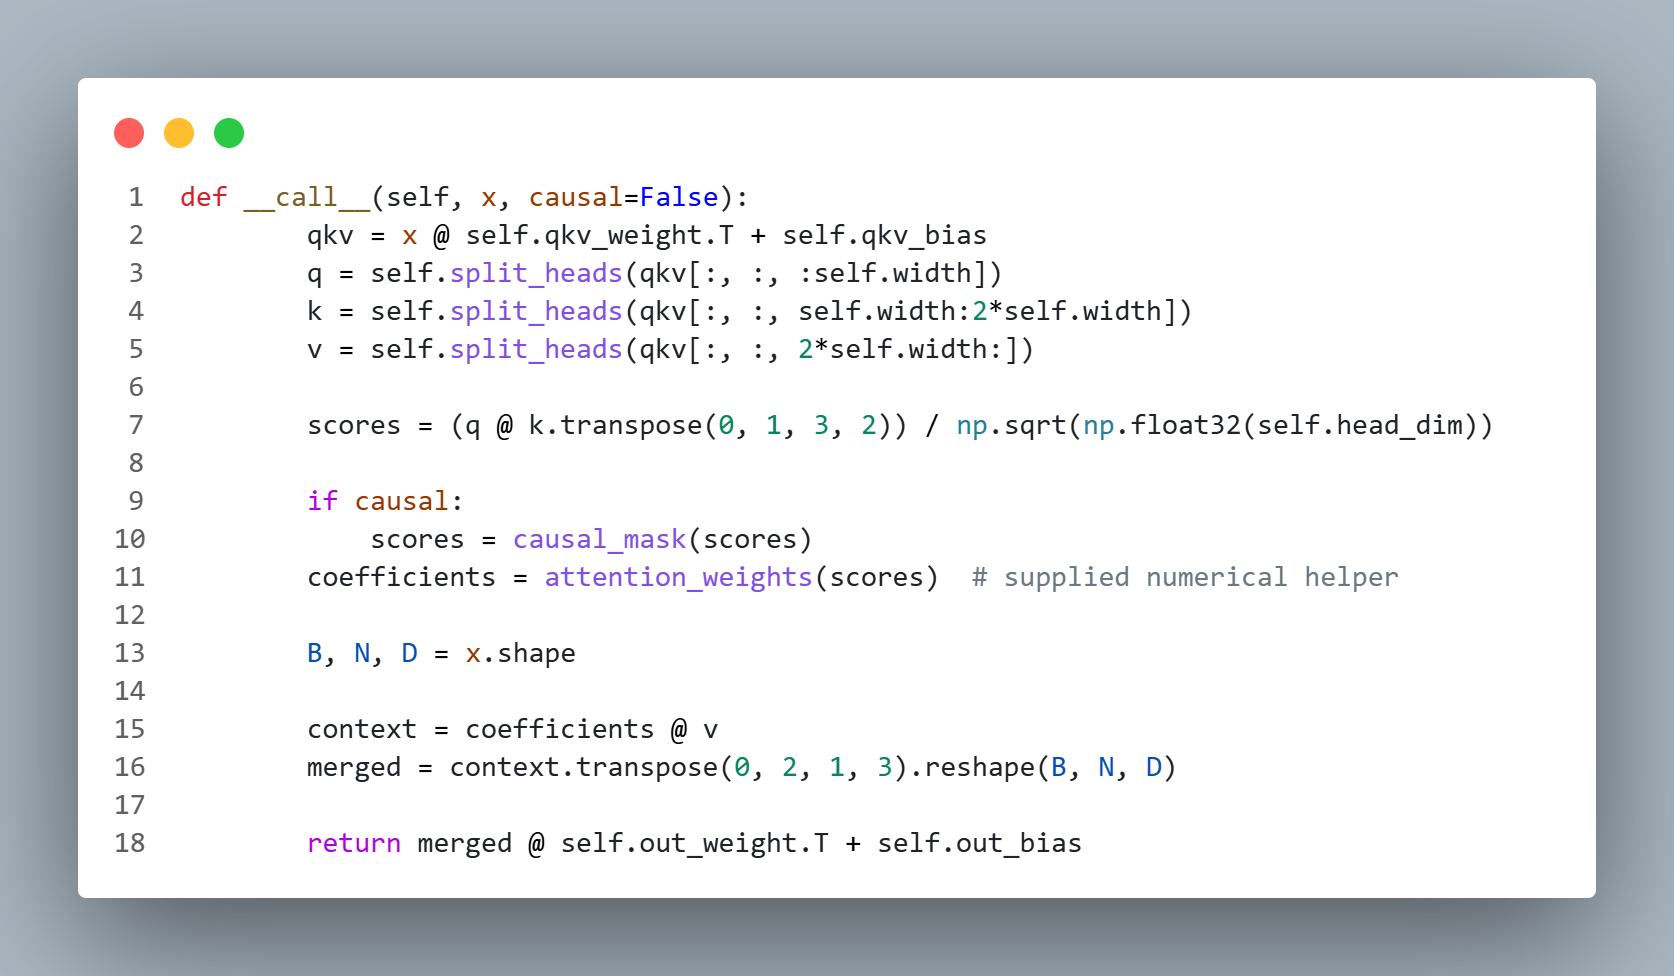
\includegraphics[width=\linewidth]{../image/todo3.png}
    \caption*{(a) TODO-03：多头注意力}
  \end{minipage}\hfill
  \begin{minipage}[t]{0.49\linewidth}
    \centering
    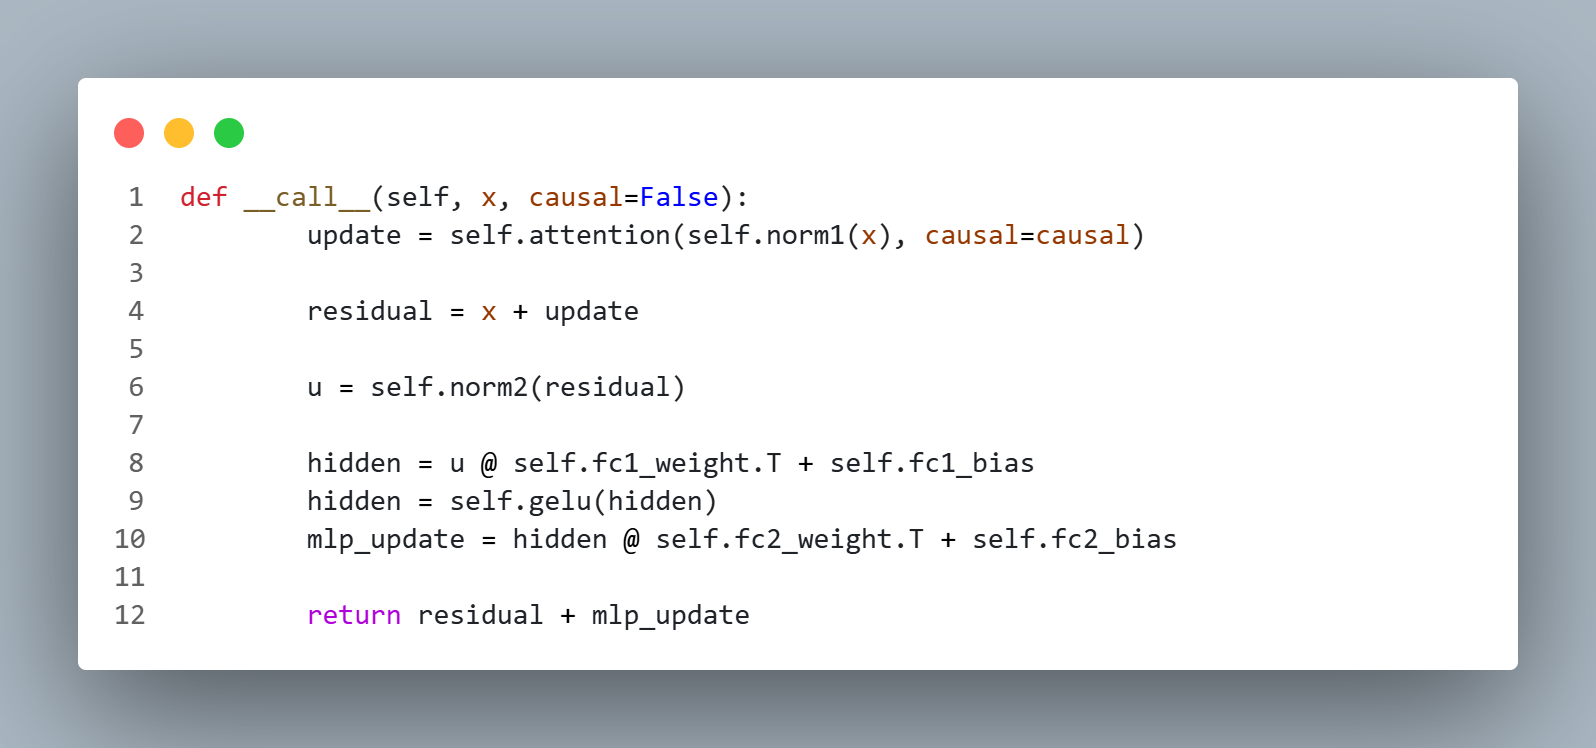
\includegraphics[width=\linewidth]{../image/todo4.png}
    \caption*{(b) TODO-04：残差连接与 MLP}
  \end{minipage}
  \caption{注意力计算和 Transformer 块的实现}
  \label{fig:todo34}
\end{figure}

\subsection*{Token 嵌入与最终输出}

图像块经过无偏置投影后得到 $[B,49,768]$，随后在 token 轴最前面拼接 CLS token，并通过广播加上位置嵌入，形成 $[B,50,768]$。
在 12 层 Transformer 计算完成后，取第 0 个 CLS token，依次进行了后置 LayerNorm、$768\to512$ 投影和单位长度归一化。

\begin{figure}[H]
  \centering
  \begin{minipage}[t]{0.49\linewidth}
    \centering
    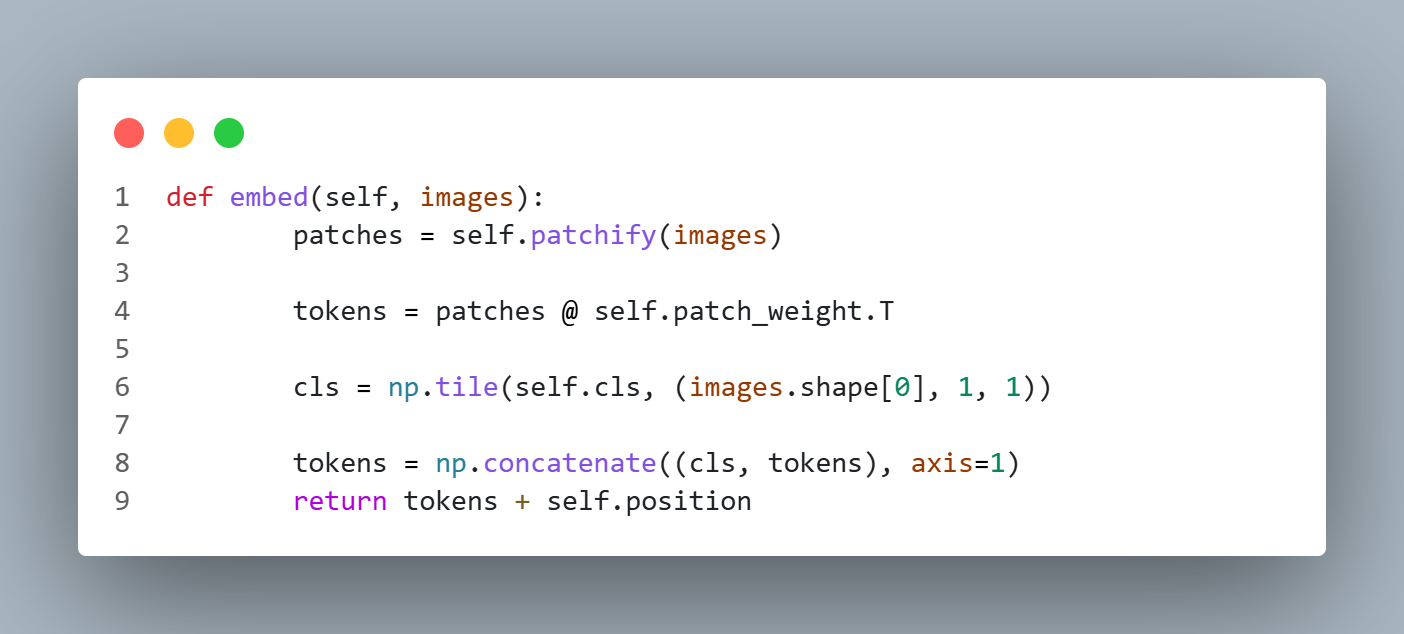
\includegraphics[width=\linewidth]{../image/todo5.png}
    \caption*{(a) TODO-05：token 嵌入}
  \end{minipage}\hfill
  \begin{minipage}[t]{0.49\linewidth}
    \centering
    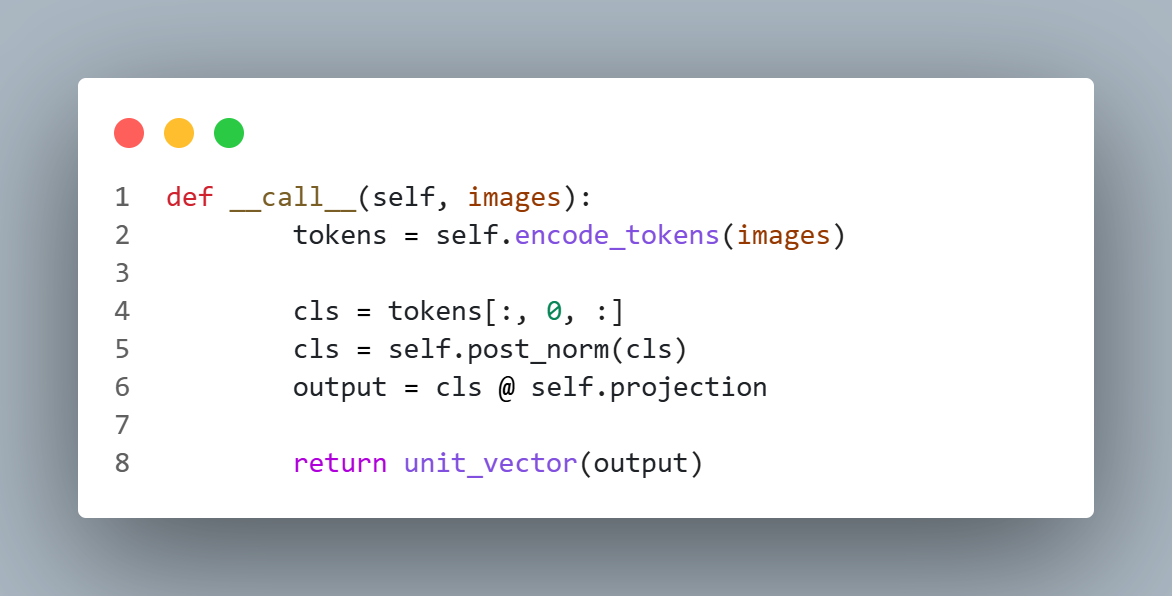
\includegraphics[width=\linewidth]{../image/todo6.png}
    \caption*{(b) TODO-06：CLS 输出}
  \end{minipage}
  \caption{输入 token 构造和最终输出的实现}
  \label{fig:todo56}
\end{figure}

\begin{table}[H]
  \centering
  \small
  \caption{各阶段与参考数组的数值误差}
  \label{tab:errors}
  \begin{tabular}{lccc}
    \toprule
    阶段           & 输出形状             & 最大绝对误差                 & 平均绝对误差                 \\
    \midrule
    preprocess   & $(10,3,224,224)$ & $0.000\mathrm{e}{+00}$ & $0.000\mathrm{e}{+00}$ \\
    patches      & $(2,49,3072)$    & $0.000\mathrm{e}{+00}$ & $0.000\mathrm{e}{+00}$ \\
    tokens       & $(2,50,768)$     & $4.005\mathrm{e}{-05}$ & $1.289\mathrm{e}{-06}$ \\
    block0       & $(2,50,768)$     & $7.063\mathrm{e}{-06}$ & $3.250\mathrm{e}{-07}$ \\
    last\_tokens & $(2,50,768)$     & $4.768\mathrm{e}{-05}$ & $2.696\mathrm{e}{-06}$ \\
    output       & $(10,512)$       & $5.439\mathrm{e}{-07}$ & $8.311\mathrm{e}{-08}$ \\
    batch        & $(3,512)$        & $4.619\mathrm{e}{-07}$ & $7.632\mathrm{e}{-08}$ \\
    \bottomrule
  \end{tabular}
\end{table}

\section{实验结果}

在项目目录执行 \texttt{check.py}。
图~\ref{fig:check} 是本次实际运行保存的终端截图。
程序通过了资产、预处理、中间 token、最终输出和改变 batch 顺序等全部检查。
误差均在合理范围内，因此我们认为实验复现是成功的。
随后利用 \texttt{run.py} 导出 \texttt{output\_tokens.npz}，成功保存形状为 $(10,512)$ 的输出数组。



\begin{figure}[H]
  \centering
  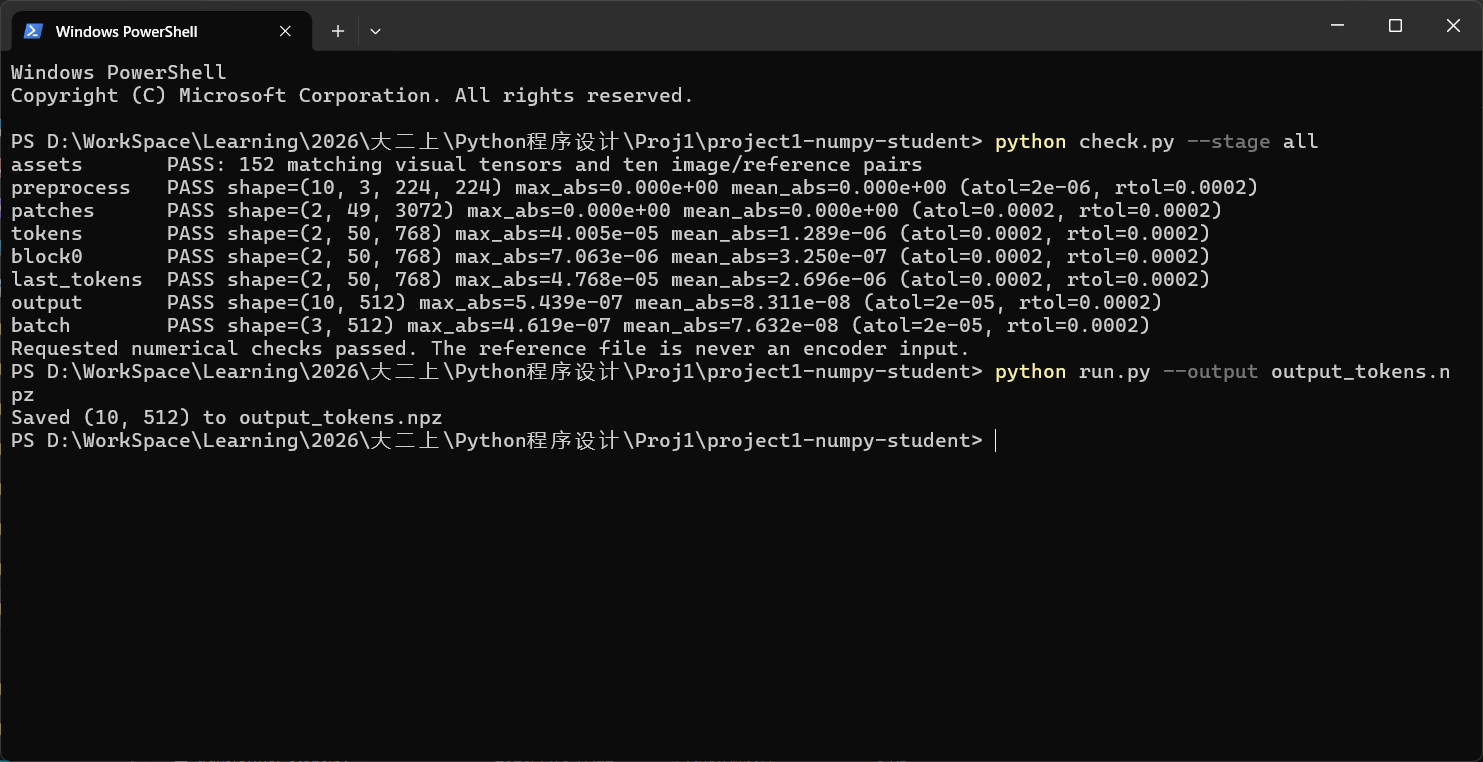
\includegraphics[width=0.94\linewidth]{../image/check.png}
  \caption{完整数值检查及输出文件生成结果}
  \label{fig:check}
\end{figure}

\section{分析与讨论}

\textbf{} 在划分图像块时，我曾把通道轴合并到图像块数量中，得到 147 个块，
但这和要求的 49 个包含 RGB 三通道的图像块矛盾。因此我重排了维度顺序，才得到正确的 $[B,49,3072]$。
这一问题说明我们要检查张量维度的排序和形状，同时确认每个轴代表的对象。

\textbf{数值结果分析。} 预处理和 \texttt{patches} 阶段与参考结果完全一致，
最大绝对误差均为 0。内部阶段允许的绝对误差为 $2\times10^{-4}$，实际最大误差不超过 $4.768\times10^{-5}$；
最终 \texttt{output} 阶段允许的绝对误差为 $2\times10^{-5}$，实际最大误差为 $5.439\times10^{-7}$，
约为该阈值的 $1/37$。所有阶段均通过形状、数据类型、有限值和 \texttt{np.allclose} 检查，
这说明了实现与独立 FP32 参考结果高度一致，我们可以认为实验成功复现了。
\texttt{batch} 检查还改变了图像顺序并包含重复图像，结果仍通过，说明程序能够处理不同顺序和重复输入，
而不是依赖固定顺序返回结果。

\textbf{参考结果评估。} \texttt{check.py} 会读取初始给出的期望输出参数，
分别计算当前实现的中间结果和最终输出，再用 \texttt{np.allclose} 比较。参考数组仅用于检查，
不会作为编码器输入。

\textbf{AI 辅助说明。} 本实验使用 GPT 6 Astra 辅助调试，并帮助理解深度学习和数值计算相关概念，协助完成 \LaTeX 排版。
核心实验、代码和测试由个人完成。

\newpage

% ============================================================
% 批阅与成绩评定页
% ============================================================

% 绘制正文外框（包含批阅区域）
\begin{tikzpicture}[remember picture, overlay]
  \draw[thick]
  ($(current page.north west)+(2cm,-3cm)$)
  rectangle
  ($(current page.south east)+(-2cm,3.5cm)$);
\end{tikzpicture}

\vspace{1cm}

% 批阅区
\noindent \textbf{指导教师批阅意见：}
\vspace{6cm}
\hfill

\vspace{1cm}

\noindent \textbf{成绩评定：}
\vspace{2cm}
\hfill

\vspace{1cm}

\noindent
\hfill
\textbf{指导教师签字：}\quad\quad\quad\quad\quad\\[0.5cm]

\hfill
\textbf{年}\quad\quad
\textbf{月}\quad\quad
\textbf{日}\quad

\vspace{1cm}

% 备注部分
\noindent \textbf{备注：}

% 框外的注释
\begin{tikzpicture}[remember picture, overlay]
  \node[
    anchor=north west,
    inner sep=0pt,
    text width=\dimexpr\paperwidth-4cm\relax
  ] at ($(current page.south west)+(2cm,3.1cm)$) {
    \begin{minipage}{\dimexpr\paperwidth-4cm\relax}
      \small
      \noindent
      \textbf{注：}\;1、报告内的项目或内容设置，可根据实际情况加以调整和补充。\\[0.2cm]
      \phantom{\textbf{注：}\;}2、教师批改学生实验报告时间应在学生提交实验报告时间后 10 日内。
    \end{minipage}
  };
\end{tikzpicture}

% ============================================================
%                      文档结束
% ============================================================

\end{document}
